\chapter{実装}
\label{implementation}

\ref{kadai}を踏まえつつ\ref{propsed}で解決に近づけるために、本章では3つの実験とその設定内容について述べる。

本章では本研究における実装環境,提案手法の実装,提案手法の評価に用いるデータセットについて述べる.
\ref{impl_env}では本研究における実験のための実行環境及び事前知識について述べる。
\ref{exp_common}では、K-AFの性能を最も引き出す可能性がある、学習の設定を調査する。
\ref{exp1}ではK-AFの性能を既存の活性化関数と比較する実験を行う。
\ref{exp2}では各データセットにおいての活性化関数の形を調査する実験をこなう。
\ref{exp3}では、K-AFの性能を最も引き出す可能性がある、学習の設定を調査する。

これら3つの実験を踏まえて、K-AFの課題に対しての実用性だけでなく、K-AFの性質についても調査し、今後の発展のための鍵となる結論へとつなげる。



\section{実装環境}
\label{impl_env}



本研究において利用した実装環境を \ref{impl_table} に示す. 提案手法の実装は Pytorch 及
を用いた.  PyTorch~\cite{pytorch}, Chainer~\cite{chainer},  Tensorflow~\cite{tensorflow} は計算グラフの自動微分ライブラリであり, 深層ニューラルネットワークの研究や開発にも用いられる.
Pytorchを用いた理由は実装コストが低く研究領域に従事できるところにある。


\begin{table}[htbp]
\label{impl_table}
    \begin{center}
        \caption{本研究の実行環境}
        \vspace{5mm} 
        \begin{tabular}{l*{2}{c}r}
        環境              & バージョン \\
        \hline
        CPU               & Intel core i7 6コア 2.2GHz \\
        メモリ             & 16GB \\
        Python            & 3.8.5  \\
        scikit-learn      & 0.23.2\\
        numpy             & 1.18.5 \\
        pytorch           & 2.5.0 \\
        \end{tabular}
    \end{center}
\end{table}



\vspace{-15mm} 
\section{本実験での共通項目}
\label{exp_common}

実験に用いる活性化関数の形を図\ref{k-af-net}に示す。
\begin{figure}[hbtp]
\label{k-af-net}
    \begin{center}
        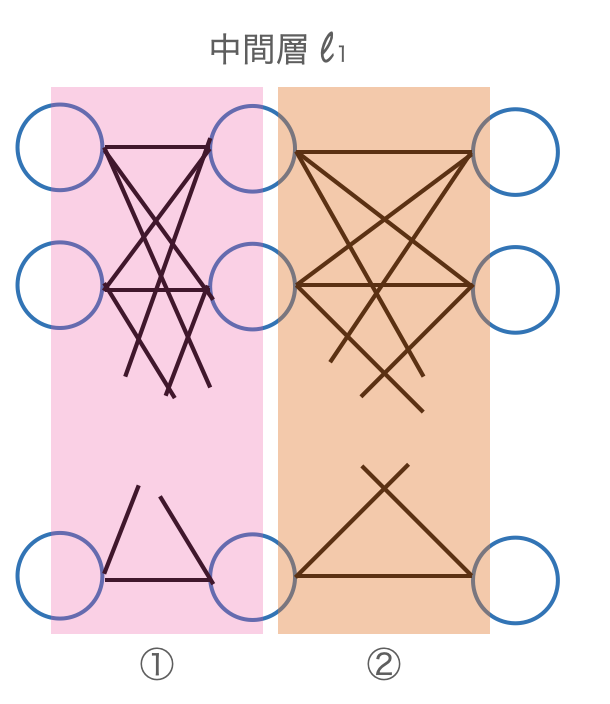
\includegraphics[width=10cm]{asset/k-af-net.png}
            \caption{実験で使うニューラルネットワークの概要図}
            \label{neural_network1}
    \end{center}
\end{figure}

今回の実験では、簡易的なモデルで活性化関数の性能を試していく。
中間層の数を$ l_1 $とし、\textcircled{\scriptsize 1}にはReLUを用いる。\textcircled{\scriptsize 2}の部分を可変的にさまざまな活性化関数へと変えていく。
本論文で提案する、K-AFは\textcircled{\scriptsize 2}の部分において性能を評価する。

比較用の活性化関数には以下を用いる。
\begin{itemize}
\label{list:active}
    \setlength{\parskip}{0cm} % 段落間
    \setlength{\itemsep}{0cm} % 項目間
    \item ReLU
    \item Sigmoid
    \item Linear
    \item Tanh
    \item Mish
    \item Swish
    \item K-AF(本手法)
\end{itemize}


活性化関数の性能の比較実験のために、以下の項目を変えながら実験する。データセットにはsckit-learn~\cite{scikit-learn}のライブラリのデータセットに対してデフォルトで入ってるものを想定する。
各種データセットの詳細については\url{https://scikit-learn.org/stable/datasets/toy_dataset.html}こちらのページが参考になる。

\begin{itemize}
\label{exp_list}
    \setlength{\parskip}{0cm} % 段落間
    \setlength{\itemsep}{0cm} % 項目間
    \item LearningRate(lr) [ $10^{-5}$, $10^{-6}$ ,$10^{-7}$]
    \item Initializer [ Xavier, kaiming uniform]
    \item Regularizer [ 何もなし, L1ノルム, L2ノルム]
    \item Optimizer [ SGD, Momentum, AdaGrad, Adam]
    \item データセット [ iris, digits, wine, boston, breast\_cancer ]
\end{itemize}

\subsection{比較データ}

他の活性化関数と適当に比較するために、以下の条件を比較して実験を行う。


\begin{table}[htbp]
    \begin{center}
        \caption{実験のデータセットの名称}
        \label{dataset_name}
        \vspace{5mm} 
        \begin{tabular}{ |c|c|c|c|c|c| }
        データセット名 & サンプル数 & 入力の次元 & 出力の次元 & 出力の形式 & 中間層の数 $ {l_1} $ \\
        \hline
        iris           & 150    & 3         & 3        & 分類      & 4 \\
        digits         & 1797   & 3         & 64       & 分類      & 100 \\
        wine           & 178    & 3         & 13       & 分類      & 40 \\
        boston         & 506    & 13        & 1        & 回帰      & 20 \\
        breast\_cancer & 569    & 30        & 2        & 分類      & 30 \\
        \end{tabular}
    \end{center}
\end{table}


\subsection{実装における留意点}
実験のために必要なハイパーパラメータとして以下のパラメータを実験前に設定することとした。

\begin{table}[htbp]
    \begin{center}
        \caption{実験のデータセットの名称}
        \vspace{5mm} 
        \scalebox{0.7}[0.7]{
            \begin{tabular}{||c | c |c||}
            ハイパーパラメータ & 説明 \\
            \hline
            epoch数                           & epoch\_num      & 学習の速度、最終的なval-Lossを見るのに十分なepoch数を取る。  \\
            実験回数                           & exp\_num     & 数回実験を行なった平均をとり、結果を保証する。 \\
            カーネル密度推定に使うデータ数        & calc\_num           & $ \mathbf{X}^{calc} $ に使うデータ数を表す。  \\
            \end{tabular}
        }
    \end{center}
\end{table}





\vspace{-15mm} 

\section{実験1 既存の活性化関数との比較実験}
\label{exp1}
\subsection{実装手法}

\ref{exp_list}に記述した5つのデータセットを軸に\ref{list:active}の活性化関数での比較実験を
学習率 、Optimizer、Initializer、Regularizerを変更しながら実験した。
K-AFの性能が有利にならないように、可能な限り任意の組み合わせで実験を行い性能の評価を行う。



\subsection{評価手法}

回帰問題と分類問題におけるれぞれの評価時における精度指標(Metrics)として、
回帰問題では平均絶対誤差(MAE)を、分類問題では正解率(Accuracy)を用いる。
これらは、最も基礎的で一般的な評価関数(Metric function)である。




\subsubsection{irisでの比較実験}
\label{impl:iris}

irisはアヤメの分類問題であり、統計学の分野で最も一般的に性能評価がおなわれるものである。
optimzerにSGD、Regularizerを特に使わない理由はirisは単純なデータセットのため、収束することを前提に考えているからである。

\begin{table}[htbp]
    \begin{center}
        \caption{irisでの実験と設定}
        \vspace{5mm} 
        \begin{tabular}{ |c|c|c| }
        設定名 & 設定1 & 設定2 \\
        \hline
        学習率(lr)         & $ 10^{-5} $ & $ 10^{-6} $ \\
        Initializer       & Xavier &  kaiming uniform \\
        Optimizer           & SGD & SGD \\
        Regularizer     & なし & なし \\
        epoch\_num       & 1 &  1 \\
        exp\_num         & 1 & 1 \\
        calc\_num        & 1 & 1 \\
        \end{tabular}
    \end{center}
\end{table}



\subsubsection{digitsでの比較実験}
\label{impl:digits}

digitsは数字の画像の分類問題であり、機械学習の分野で一般的に性能評価の対象として使用されるものである。
digitsは次元数が高いデータセットであるため、OptimizerにはAdamとSGD, レギュライザーにはL1とL2を使用した。

\begin{table}[htbp]
    \begin{center}
        \caption{digitsでの実験と設定}
        \vspace{5mm} 
        \begin{tabular}{ |c|c|c| }
        設定名 & 設定1 & 設定2 \\
        \hline
        学習率(lr)         & $ 10^{-5} $ & $ 10^{-6} $ \\
        Initializer       & Xavier & kaiming uniform \\
        Optimizer           & SGD & Adam \\
        Regularizer     & L1 & L2 \\
        epoch\_num       & 1 &  1 \\
        exp\_num         & 1 & 1 \\
        calc\_num        & 1 & 1 \\
        \end{tabular}
    \end{center}
\end{table}



\subsubsection{wineでの比較実験}
\label{impl:wine}

wineとはワインの種類の判別を13個の入力次元の性質を用いて3つにカテゴライズするデータセットである。
主に決定木の性能評価に使われることが多い。本実験では以下のデータセットを用いて行う。

\begin{table}[htbp]
    \begin{center}
        \caption{wineでの実験と設定}
        \vspace{5mm} 
        \begin{tabular}{ |c|c|c| }
        設定名 & 設定1 & 設定2 \\
        \hline
        学習率(lr)         & $ 10^{-5} $ & $ 10^{-6} $ \\
        Initializer       & Xavier & kaiming uniform \\
        Optimizer           & SGD & Adam \\
        Regularizer     & L1 & なし \\
        epoch\_num       & 1 &  1 \\
        exp\_num         & 1 & 1 \\
        calc\_num        & 1 & 1 \\
        \end{tabular}
    \end{center}
\end{table}


\subsubsection{bostonでの比較実験}
\label{impl:boston}

bostonはボストンの住宅価格を回帰で推定する問題である。K-AFが回帰問題に対しても有効であることを示すため、この実験を行う。

\begin{table}[htbp]
    \begin{center}
        \caption{bostonでの実験と設定}
        \vspace{5mm} 
        \begin{tabular}{ |c|c|c| }
        設定名 & 設定1 & 設定2 \\
        \hline
        学習率(lr)         & $ 10^{-5} $ & $ 10^{-6} $ \\
        Initializer       & Xavier & kaiming uniform \\
        Optimizer           & SGD & Adam \\
        Regularizer     & L1 & なし \\
        epoch\_num       & 1 &  1 \\
        exp\_num         & 1 & 1 \\
        calc\_num        & 1 & 1 \\
        \end{tabular}
    \end{center}
\end{table}

\vspace{-15mm} 


\subsubsection{breast\_cancerでの比較実験}
\label{impl:breastcancer}

breast\_cancerは乳がんのデータセットである。

\begin{table}[htbp]
    \begin{center}
        \caption{breast\_cancerでの実験と設定}
        \vspace{5mm} 
        \begin{tabular}{ |c|c|c| }
        設定名 & 設定1 & 設定2 \\
        \hline
        学習率(lr)         & $ 10^{-5} $ & $ 10^{-6} $ \\
        Initializer       & Xavier & kaiming uniform \\
        Optimizer           & SGD & Adam \\
        Regularizer     & L1 & なし \\
        epoch\_num       & 1 &  1 \\
        exp\_num         & 1 & 1 \\
        calc\_num        & 1 & 1 \\
        \end{tabular}
    \end{center}
\end{table}


\vspace{-5mm} 

\section{実験2 K-AFの関数形状の調査}
\label{exp2}

2つ目の実験では推論した活性化関数の形を\ref{dataset_name}に記載したデータセット観測し、既存の活性化関数との違いを定性評価を行う。
活性化関数の種類を分割すると以下のようになっている。
また、ニューラルネットワークの設定は\ref{exp1}の設定で各データセットごとに二つずつ結果を取得する。

\begin{table}[htbp]
    \begin{center}
        \caption{活性化関数の関数的な意味}
        \label{af-class}
        \vspace{5mm} 
        \begin{tabular}{ |c|c|c| }
        単調増加関数か & 勾配が$ 0 $の点があるか & 上限値があるか   \\
        \hline
        ○ or × & ○ or × & ○ or ×  \\
        \end{tabular}
    \end{center}
\end{table}

\vspace{-5mm} 

\ref{af-class}を軸に、K-AFの形状を分析し、既存の活性化関数と比べて何が違うか評価を行う。






\section{実験3 K-AFの性能が上がる条件探査}
\label{exp3}
各種データセットのでK-AFでの結果を出す前に、K-AFが一般的にどのような場合に性能を出しやすいか\ref{exp_list}での設定をランダムに組み合わせて、どの結果が一番性能が出たか評価する。
実験1ではデータセットとしてirisとdigitsにおいて性能評価を行う。その際のニューラルネットワークの設定は\ref{dataset_name}を軸に設定する。
他に実験において必要なパラメータを以下に設定する。


\begin{table}[htbp]
    \begin{center}
        \caption{実験のデータセットの名称}
        \vspace{5mm} 
        \scalebox{0.7}[0.7]{
            \begin{tabular}{||c | c |c||}
              & irisの場合 & digitsの場合 \\
            \hline
            epoch数                           & 200       & 200  \\
            実験回数                           & 10     & 10 \\
            カーネル密度推定に使うデータ数        & 50           & 50  \\
            \end{tabular}
        }
    \end{center}
\end{table}


\vspace{-15mm} 








%%% Local Variables:
%%% mode: japanese-latex
%%% TeX-master: "../bthesis"
%%% End:
